\documentclass[12pt,a4paper]{report}
\usepackage[utf8]{inputenc}
\usepackage{colortbl}
\usepackage{url}
\usepackage{fancyhdr}
\usepackage[margin=1in]{geometry}
\usepackage{lipsum}
\usepackage{times}
\usepackage{graphicx}
\usepackage{multirow}
\graphicspath{ {images/} }
\usepackage{wrapfig}
\usepackage{rotating}
\usepackage[singlelinecheck=false,justification=Centering]{caption}

\linespread{1.5}
\setlength{\parindent}{6ex}
\usepackage{float}
\usepackage{indentfirst}
\usepackage{color, colortbl}
\usepackage{caption} 
\setcounter{secnumdepth}{3}
\setcounter{tocdepth}{3}
\usepackage{pdfpages}
\renewcommand{\contentsname}{\centering Table of Contents}
\definecolor{LightCyan}{rgb}{0.88,1,1}
\usepackage{titletoc}
%\titlecontents{section}[left]{above-code}{numbered-entry-format}{numberless-entry-format}{filler-page-format}[below-code]
\newcommand{\setupname}[1][\chaptername]{
	\titlecontents{chapter}[0pt]{\vspace{1ex}}{\bfseries#1~\thecontentslabel:\quad}{\bfseries}{\bfseries\hfill\contentspage}[]
}
\begin{document}

	
	\pagenumbering{roman}   %set page numbering to roman%	
	\setcounter{page}{1}
	
	\chapter*{\centering Acknowledgment}
	\addcontentsline{toc}{chapter}{Acknowledgement}
	
	I would like to express my deepest appreciation to all those who aide me to complete this report.  A special gratitude is giving to my final year project  manager, Mr. \textsc{Bayrem TRIKI}, whose contribution in stimulating suggestions and encouragement,  helped me to coordinate this project especially in writing this report. And a special thanks goes to my supervisor Mr. \textsc{Anis Ben Bettaieb}, who guided me throughout the development of  \textbf{``Cake it up !''} application.\\
	
	Furthermore I would also like to acknowledge with much appreciation the crucial role of the school EPI, who gave the permission to use all required  equipment and the necessary materials to complete this project. Finally, we have to appreciate the guidance will be given by other supervisor, especially in my project exposition that will surely improve my presentation skills thanks to their comment and advices.
	
	
	%content
	\tableofcontents
	\cleardoublepage
	\addcontentsline{toc}{chapter}{\listfigurename} 
	\listoffigures	
	\cleardoublepage
	\addcontentsline{toc}{chapter}{\listtablename} 
	\listoftables	
	\clearpage 
	
	\pagenumbering{arabic} 
	\setcounter{page}{1}
	
	
	\chapter*{\centering General introduction}
	\addcontentsline{toc}{chapter}{General introduction}
	Bakeries are a popular type of foodservice establishment, and they allow you to express your culinary creativity while also serving a unique market, the problem is you can spend all day and night in the kitchen creating the next best cake, but if no one knows about it, it doesn’t matter.  \par 
	In order to succeed in the bakery business,  some marketing and advertising can make a big difference.\par
	
	Depending on all of that, our application named \textbf{``Cake it up !''} have to fill in the needs of both parts the business owner and the client. It needs an easy way for the owner to promote their business and easier way for the client to find a place that matches him.\par
	This report contains three chapters; the first chapter will be taking over the project specification, presenting the problematics and their solutions. The second chapter will be concerned about conception, different diagrams; class and sequence. Then we will proceed in the realization of the application as a third chapter which in it we will talk about the used technologies, architecture and the implementation. Last but not least, the general conclusion which will give a general and brief idea on what we did throughout this report.\par
	
	\pagestyle{fancy}
	\fancyhf{}
	\fancyhead[LE,RO]{\leftmark}
	\fancyfoot[CE,CO]{\thepage}
	\renewcommand{\footrulewidth}{0.4pt}
	\setupname
	\chapter{Preliminary Study }
	\section*{Introduction}
	\addcontentsline{toc}{section}{Introduction}
	This chapter is dedicated to list the different obstacles that a business owner and a client face, which will guide us to give details on the proposed solution followed by the specification of the project. We will also introduce both the project life cycle and the used methodology. We will also give a detailed description of the use case diagram and the system sequence diagram. Finally we will end this section by a conclusion.
	
	\section{Analysis of the existing}
	We are in an era where technology leads everything, there is an application for most of the people's needs, however most of these softwares lack some details that are not yet fulfilled.\par
	This section will start by listing some of the applications or ways people use to get information about pastries, then criticize every one of them to show what is missing.
	\subsection{Social media}
	The mostly common way is using the social media such as \textbf{``FACEBOOK''} and \textbf{``INSTAGRAM''} where you can find a verity of choices and number of opinions that can guide the user to select the right place.\par We can also use it to figure out the cost of the meal or get direction as shown in Figure \ref{label-facebook}.
	\par The social media also give you the ability to communicate with the manager of the place in private to either pass an order or to ask for more details regarding a specific product.  \par
	\begin{figure}[H]
		\centering
		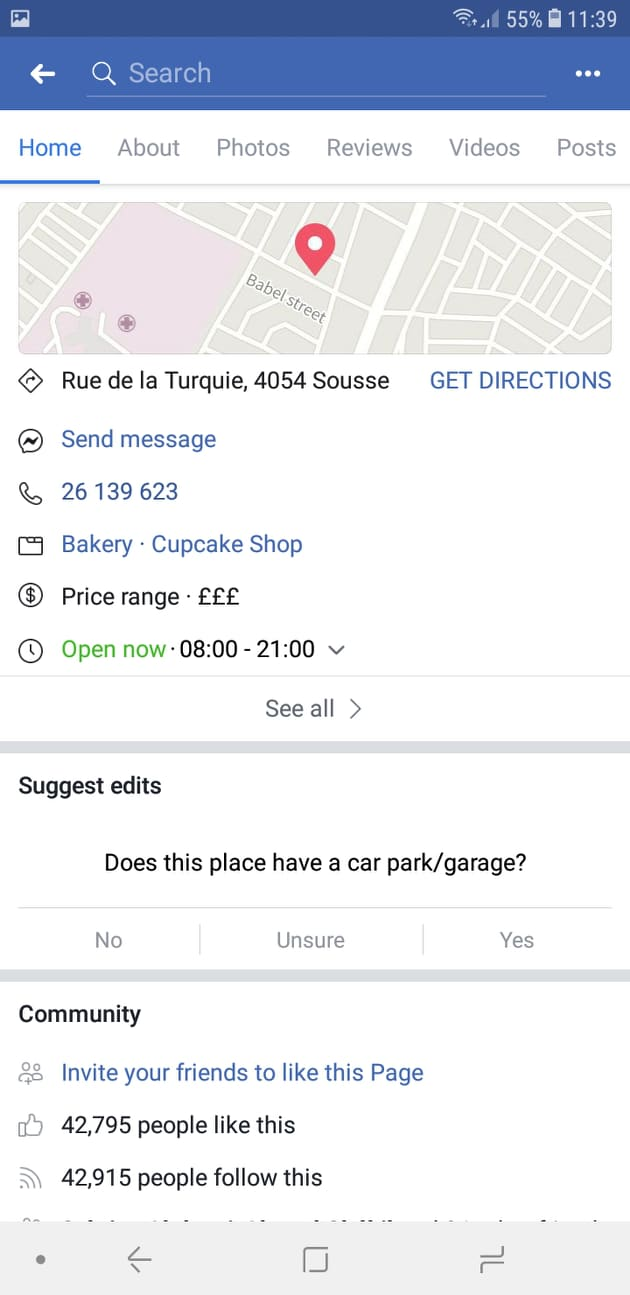
\includegraphics[width=3in,keepaspectratio]{facebook.jpg}
		\caption{Application: FACEBOOK\protect\refstepcounter{footnote}\protect\footnotemark[\thefootnote]}
		
		\label{label-facebook}
	\end{figure}
	\footnotetext[\thefootnote]{Source: https://www.facebook.com/}
	\clearpage
	\subsection{Google maps}
	\textbf{``Google maps''} has been popular for quite a while now, it can be used to figure out the nearby pastries, reviewing shop and get directions as showing in Figure \ref{label-googlemaps}. \par
	\begin{figure}[H]
		\centering
		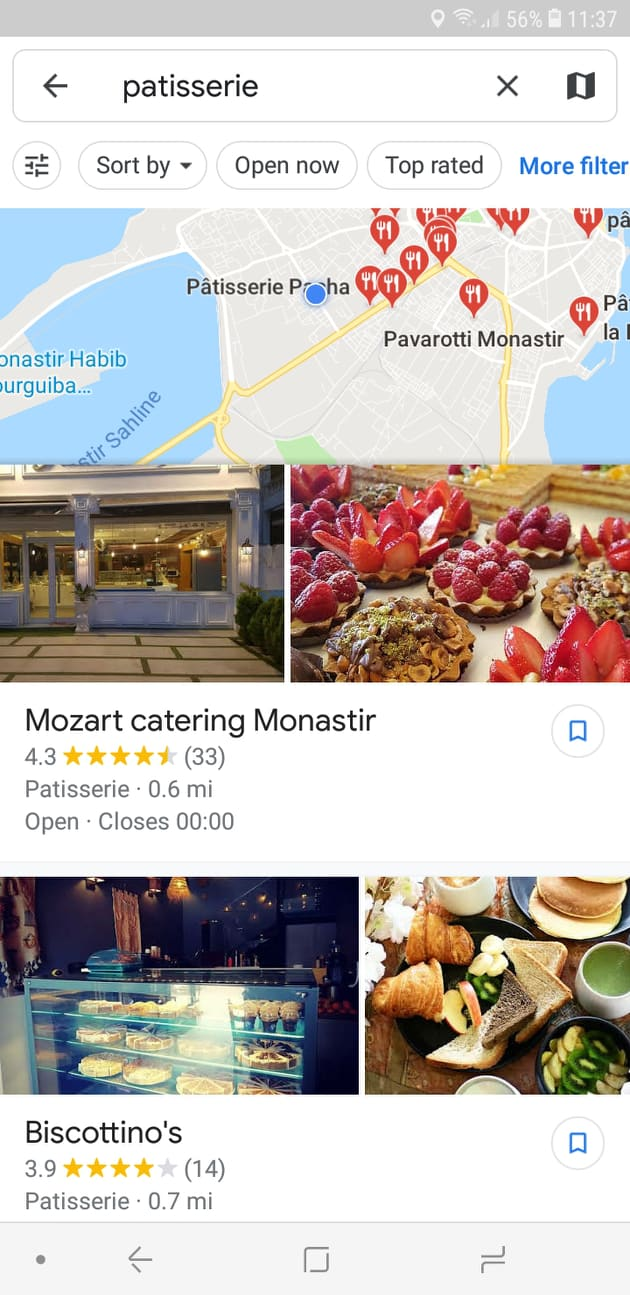
\includegraphics[width=3in,keepaspectratio]{googlemaps.jpg}
		\caption{Google maps\protect\refstepcounter{footnote}\protect\footnotemark[\thefootnote]}
		
		
		
		\label{label-googlemaps}
	\end{figure}
	\footnotetext[\thefootnote]{Source: https://www.google.com/maps}
	\clearpage
	\subsection{Bakery days}
	\textbf{``Bakery days''} gives you the ability to design your cake as presented in Figure  \ref{label-zomato}:
	
	
	\begin{figure}[H]
		\centering
		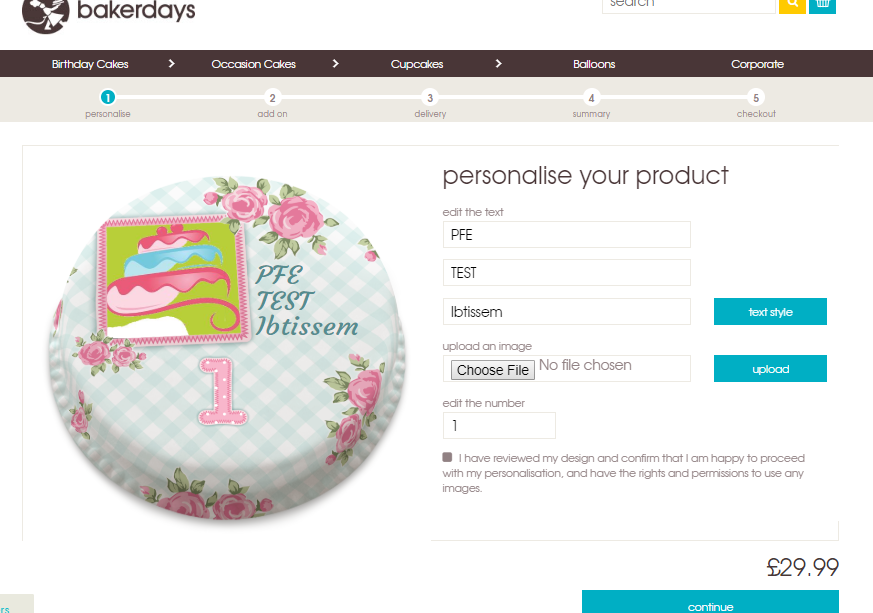
\includegraphics[width=7in,keepaspectratio]{bakerydays.png}
		\caption{Web site: Bakery days\protect\refstepcounter{footnote}\protect\footnotemark[\thefootnote]}
		
		\label{label-zomato}
	\end{figure}
	\footnotetext[\thefootnote]{Source: https://www.bakerdays.com/}
	\subsection{YELP}
	\textbf{``Yelp''} has tremendous power in the pastries industry, and having a strong backing of positive Yelp reviews is like having a flock of golden geese reviews from Yelp can do wonders for any business.\par 
	Advantages of \textbf{``Yelp''}:
	\begin{itemize}
		\item The application provide two parts, the business owner's section presented in Figure \ref{label-yelp1} and the visitor in Figure \ref{label-yelp2}.
		\item  The user can add his own business by adding as many details as possible.
		\item He can respond to the reviews.
		\item Manage his shop.
		\item A visitor can rate and review a shop.
		
	\end{itemize}
	\begin{figure}[H]
		\centering
		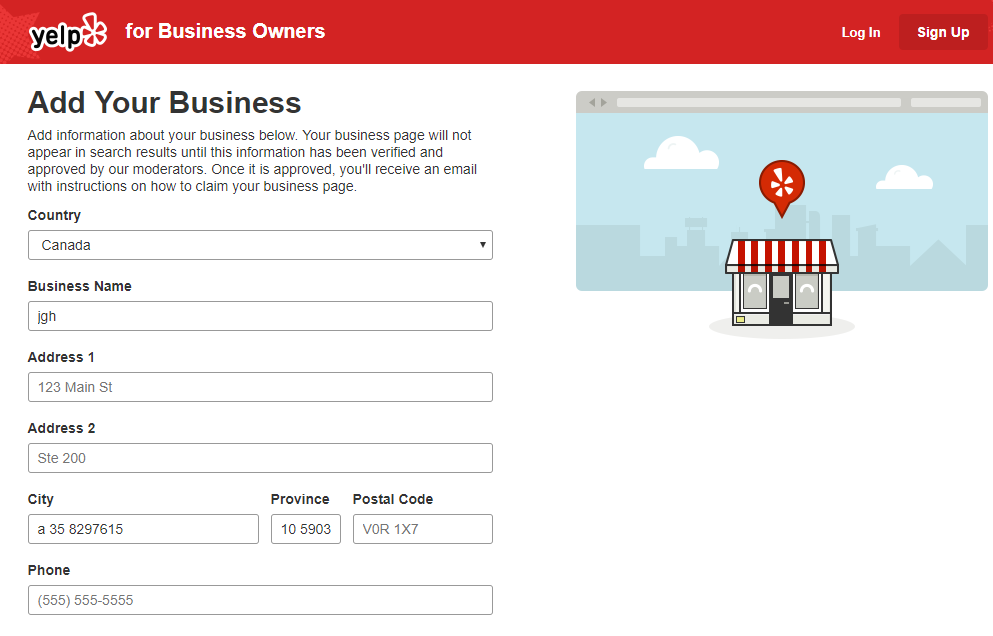
\includegraphics[width=5in,keepaspectratio]{yelp.png}
		\caption{Web application: Yelp (business owner)\protect\refstepcounter{footnote}\protect\footnotemark[\thefootnote]}
		
		
		\label{label-yelp1}
	\end{figure}
	\footnotetext[\thefootnote]{Source: https://biz.yelp.ca}
	\begin{figure}[H]
		\centering
		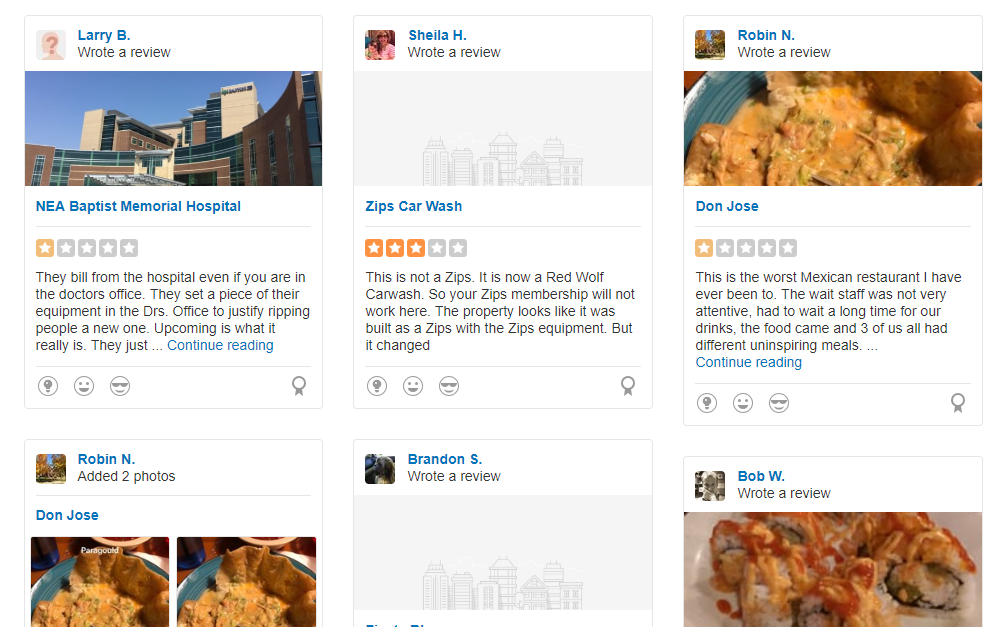
\includegraphics[width=5in,keepaspectratio]{yelp2.png}
		\caption{ Web application: Yelp (user)\protect\refstepcounter{footnote}\protect\footnotemark[\thefootnote]}
		
		
		\label{label-yelp2}
	\end{figure}
	\footnotetext[\thefootnote]{Source: https://www.yelp.com}
	\subsection{Criticism of the existing}
	As shown in Table \ref{table-criticism}, there are number of disadvantages that can not be ignored.
	\begin{table}[H]
		\begin{center}
			\captionsetup[table]{skip=10pt}
			\caption{\label{table-criticism} List of disadvantages of the existing.}
			\setlength\doublerulesep{0.5pt}
			\begin{tabular}{| l | p{13cm} |}
				\hline \hline\hline
				\rowcolor{LightCyan}
				\textbf{ Existing} & \textbf{Disadvantages} \\ \hline\hline\hline
				Social media       &                        
				\vtop{\hbox{\strut Time consuming.}\hbox{\strut  Risk of being wrongly informed about the place.}\hbox{\strut 	No information about the prices.}\hbox{\strut No security in passing orders.}}
				
				\\ \hline
				Google maps        &                        
				\vtop{\hbox{\strut Places are added by anyone not the owner.}\hbox{\strut  The suggestion are only based on the location of the user.}\hbox{\strut No on-line orders.}\hbox{\strut Not enough information about the products.}}
				
				\\ \hline
				Bakery days        &                        
				\vtop{\hbox{\strut The personal design includes only the image on the cake or the writing.}\hbox{\strut The site is for one specific bakery.}
					\hbox{\strut Only available as a web site.}
					\hbox{\strut Covers only the United Kingdom.}}
				\\
				\hline
				YELP               &                        
				\vtop{\hbox{\strut The site is designed only for reviews.}\hbox{\strut Can not pass an order.}\hbox{\strut Too many types of business.}
					\hbox{\strut Not available worldwide.}}
				\\ \hline
				
				
			\end{tabular}
			
		\end{center}
		
	\end{table}
	\clearpage
	\section{Solution and requirements}
	This section will give a small presentation of the solution regarding previous criticism followed by the requirements for this solution.
	\subsection{Proposed Solution}
	As a solution for the previous issues, I provided a web/mobile application named \textbf{``Cake it up !''}.\par
	In one hand, the mobile part will be dedicated to the clients everywhere. It provides an easier way to view all the pastries nearby or far away and get access to all their product's information (price, description, ...). In addition to that he can pass orders from his phone. He also has the capability to rate and give his own opinion about the bakeries or even block/report a shop. Finally, he can create his own cake design in 3D (forms, layers, colors, perfumes, ...). \par
	On the other hand, the web application is accessible for bakeries owners, so they can contribute by adding their place to the application with detailed description of their products (prices, ingredients, ...). The owner can also manage the orders of his clients or report any suspicious ones. The application gives also a daily statistic of the shop and its performance.
	
	\subsection{Requirements}
	The purpose of the requirements also called specifications is to give a clear picture of the application, in terms of the capability required. It will also identify constraints on the software solution, that are important in guiding decision making throughout the development process.
	\par
	Describing what the software system does and how it does so	effectively usually means describing it from more than one viewpoint. Each viewpoint will
	convey some information about the system that other viewpoints omit. We distinguish  two viewpoints Functional and non-Functional.
	\clearpage
	\subsubsection{Functional requirements}
	The Functional requirements are any requirement which specifies what the system should do.
	The application should be able to response to all the user’s needs:
	
	\begin{itemize}
		\item Web
		\begin{itemize}
			\item  Web master
			\begin{itemize}
				\item Connexion as a super Admin of the application
				\item Manage reports
				\item View statistics
				\item Activate/deactivate pastries
				\item Block clients
				\item Manage account
				\item Receive notifications
				
			\end{itemize}
			\item  Bakery manager	
			\begin{itemize}
				\item Create an account
				\item Connexion
				\item Manage shop
				\item Manage complains
				\item Manage orders
				\item View statistics
				\item Manage products
				\item Manage events	
				\item Receive notifications			
			\end{itemize}
		\end{itemize}
		\item Mobile
		\begin{itemize}
			\item Visitor
			\begin{itemize}
				\item Inscription
				\item Connexion
				\item Manage cart
				\item Consult pastries and products
			\end{itemize}
			\item Customer
			\begin{itemize}
				\item Connexion
				\item Manage account
				\item Manage orders
				\item Create complains
				\item Manage cart
				\item Add views
				\item Consult pastries and products
				\item Design a 3D cake
				\item Report a Bakery
				\item Access to history of orders
				\item Receive notifications
				\item Rate a pastry shop
			\end{itemize}
			
			
		\end{itemize}
	\end{itemize}
	
	\subsubsection{Non-Functional requirements}
	Non-Functional requirements are any requirement which specifies how the system performs a certain function. They generally specify the system’s quality attributes or characteristics.
	\begin{itemize}
		\item Security: every account is secured by a encrypted password 
		\item Performance: quick response
		\item Reliability: fault tolerance
		\item Maintainability: easy to fix and evolve
		\item Availability: the application can be used anytime and anywhere
		
	\end{itemize}
	\section{Used methodology}
	
	As a methodology we decided to use one the waterfall models which is the V-model.
	The V-Model is a unique, linear development methodology used during a Software Development Life Cycle (SDLC).\par 
	The V-Model depicted in Figure \ref{label-vmodel} offers a finer grained view of the various steps and interactions pertaining to the development process and can be regarded as the most commonly used work-flow that applies at system or software level.\\
	
	\begin{figure}[H]
		\centering
		\includegraphics[width=5in,keepaspectratio]{Vmodel.png}
		\caption{Methodology: V-Model\protect\refstepcounter{footnote}\protect\footnotemark[\thefootnote]}
		
		\label{label-vmodel}
	\end{figure}
	\footnotetext[\thefootnote]{Source: GitHub.}
	\section{Use case diagram}
	The purpose of a Use Case Diagram (UCD)\footnote{A use case diagram can summarize the details of your system's users (also known as actors) and their interactions with the system} in Unified Modeling Language (UML)\footnote{The OMG's Unified Modeling Language™ (UML®) helps you specify, visualize, and document models of software systems, including their structure and design, in a way that meets all of these requirements} is to demonstrate the different ways that a user might interact with a system.\\
	A use case helps represent: 
	
	\begin{itemize}
		\item 	Scenarios in which your system or application interacts with people, organizations, or external systems
		\item 	Goals that your system or application helps those entities (known as actors) achieve
		\item  	The scope of your system
	\end{itemize}
	
	\subsection{Actors}
	\textbf{``Cake it up !''} includes two main actors and one secondary actor. They are divided into two categories web and mobile as shown in Table \ref{table-actors}.
	\\
	\newcolumntype{l}{>{\columncolor{LightCyan}}c}
	\begin{table}[H]
		\begin{center}
			\caption{\label{table-actors} List of actors.} 
			\captionsetup[table]{skip=10pt}
			\setlength\doublerulesep{0.5pt}
			\begin{tabular}{|l|p{5cm}|p{8cm}| } 
				\hline\hline
				\rowcolor{LightCyan}
				& \textbf{Actor} & \textbf{Role}                                                                                 \\
				\hline
				\hline
				\multirow{3}{*}{\textbf{Web} }
				
				& Pastry manager & He is the owner of the pastry, he is responsible for the managing of his own bakery.          \\
				\cline{2-3}
				& Administrator  & This is a secondary actor, he has access to all the data of both web and mobile applications. \\
				\hline
				\hline
				\textbf{Mobile} & Customer/Visitor & He has only access to the mobile application.                                                 \\
				
				\hline
			\end{tabular}
		\end{center}
		
	\end{table}
	
	\subsection{Modeling Language}
	\begin{wrapfigure}{l}{0.2\linewidth}
		\centering
		
\includegraphics[width=0.8in]{uml.png}
	\end{wrapfigure}
	For the modeling language, we chose UML~\cite{fowler2004uml} short for Unified Modeling Language.\par
	UML is a standardized modeling language consisting of an integrated set of diagrams, developed to help system and software developers for specifying, visualizing, constructing, and documenting the artifacts of software systems, as well as for business modeling and other non-software systems.
	
	\subsection{Use case: web}
	This section will give a detailed description of the general and detailed use cases that exists in the web application.
		\subsubsection{General user case}
		 Figure \ref{user-case-web} shows the general use case of the web application which will be explained in Table \ref{user-case-web-explanation}.
			\begin{figure}[H]
				\vspace*{3cm}

				\centering
				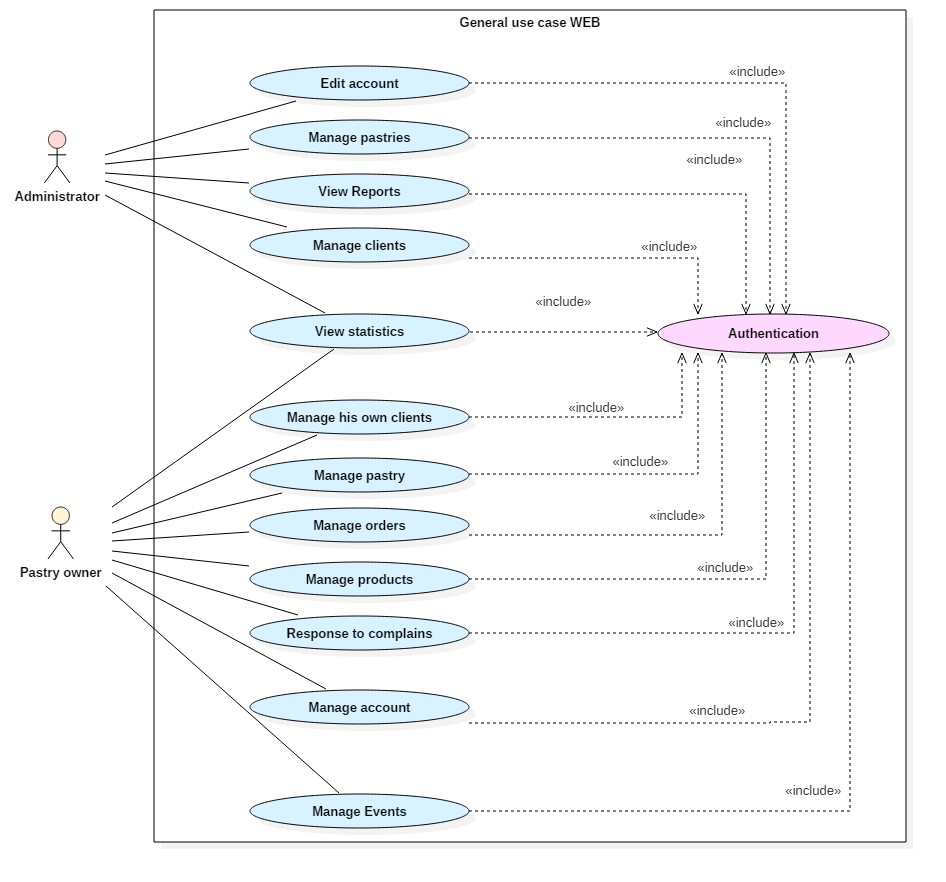
\includegraphics[width=7in,keepaspectratio]{usecaseWeb.png}
				\caption{General use case: Web}
				\label{user-case-web}
			\end{figure}
		
		\begin{table}[H]
			\begin{center}
				\caption{\label{user-case-web-explanation} General use case web explanation} 
				\captionsetup[table]{skip=10pt}
				\setlength\doublerulesep{0.5pt}
				\begin{tabular}{|l|p{5cm}|p{8cm}| } 
					\hline\hline
					\rowcolor{LightCyan}
					& \textbf{Use case} & \textbf{Explanation}                                                                                 \\
					\hline
					\hline
					\multirow{5}{*}{\textbf{Administrator} }
					
					& Edit account & The administrator has access to his own private account where he can edit his personal information,          \\
					\cline{2-3}
					& Manage pastries  & He can also view the list of all the pastries and manage them but with limits, \\
					\cline{2-3}
					& View Reports  & Viewing the reports is also an option, a report can be send from a client or a pastry, \\
					\cline{2-3}
					& Manage clients  & Managing the clients is one of the Administrator's tasks. \\
					
					\hline
					\hline
					\multirow{5}{*}{\textbf{Patsy owner} }
					& Manage his own clients & The second user which is the pastry's owner have access to the list of his clients (the ones who made at least one order with them),
					\\
					\cline{2-3}
					& Manage pastry  & He can view the information of his pastry and edit or deactivate it,
					\\
					\cline{2-3}
					& Manage orders  & All the orders made by a client can be seen by the pastry's owner, and he has multiple actions he can use on an order(accept, refuse, cancel, ...),
					\\
					\cline{2-3}
					& Manage products  & Every pastry has a list of products that are created and managed by the pastry's owner, 
					\\
					\cline{2-3}
					& Response to complains  & The complains made by the clients are only visible to this user, he has the ability to response to these complain by a message, 
					\\
					\cline{2-3}
					& Manage account  & The pastry's owner have access to his own information (email, password)\\
					\cline{2-3}
					& Manage events  & The pastry's owner have a secondary option which is handling his private calendar\\
					\hline
				\end{tabular}
			\end{center}
			
		
			\end{table}
		\subsubsection{Administrator's detailed use case diagrams}
		This section will cover some of the detailed use case diagrams for the Administrator.
			\subsubsection*{Use case: Manage Pastries}
			Figure \ref{user-case-manage-pastries} shows the detailed use case diagram for the general use case "Manage pastries". To manage the list of pastries means the Administrator has to ability to block, activate or deactivate a pastry and to see the details a specific pastry.
		\begin{figure}[H]
			\centering
			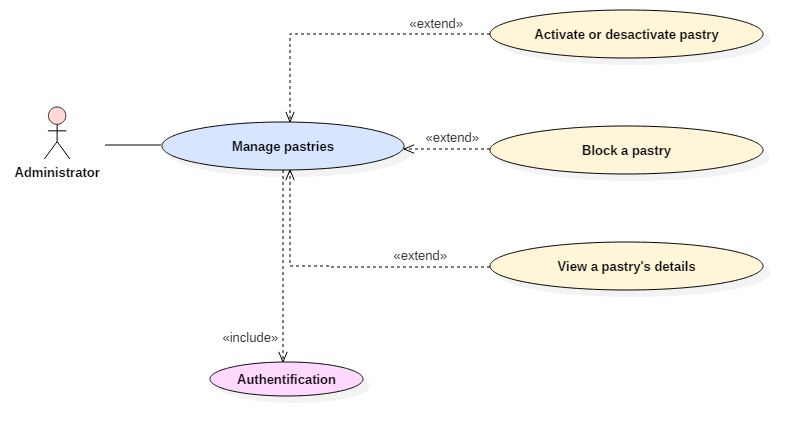
\includegraphics[width=5in,keepaspectratio]{gererPats.png}
			\caption{Detailed use case: Manage pastries}
			\label{user-case-manage-pastries}
		\end{figure}
		\subsubsection*{Use case: Manage Clients}
		The administrator can also manage the list of all the clients, he is able to block a client or view the last one's details as showing in Firgure \ref{user-case-manage-clients}.
		\begin{figure}[H]
			\centering
			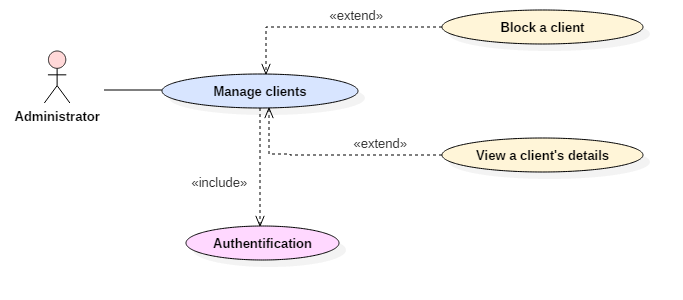
\includegraphics[width=5in,keepaspectratio]{gererClients.png}
			\caption{Detailed use case: Manage clients}
			\label{user-case-manage-clients}
		\end{figure}

		\subsubsection{Pastry manager's detailed use case diagrams }
		The pastry's manger or the pastry's owner has multiple tasks as showing in the general use case diagram, and each use case is divided into a number of other use cases.
		
		\subsubsection*{Use case: Manage his own Clients}
		After the pastry's owner authenticate, just like the Administrator, a pastry's owner can manage list of clients, the only difference is the clients list for the pastry's owner has only the clients which they passed an order with the pastry. He can report a client or view the client's information like the Figure \ref{user-case-manage-clients-pastry} shows.
		\begin{figure}[H]
			\centering
			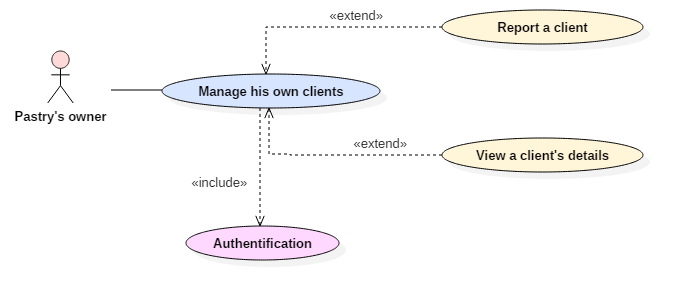
\includegraphics[width=5in,keepaspectratio]{gererClientspastry.png}
			\caption{Detailed use case: Manage his own clients}
			\label{user-case-manage-clients-pastry}
		\end{figure}
	\subsubsection*{Use case: Manage pastry}
	Figure \ref{user-case-manage-pastry} gives a detailed use case diagram of the use case 'Manage pastry', showing that a pastry's owner can desactivate his pastry which mean it will no longer be visible in the mobile application, he can consult all the details considering his pastry such as name, description, schedule, ..., from the same action he can view the list af reviews written about his pastry. 
	\par 
	Editing a pastry also has two use cases, the first one is editing all the personal information (name, description, location, ...), and the second is to change the color of the template showing on the mobile application for his pastry. None of the previous actions can be done without authentication.
	\begin{figure}[H]
		\centering
		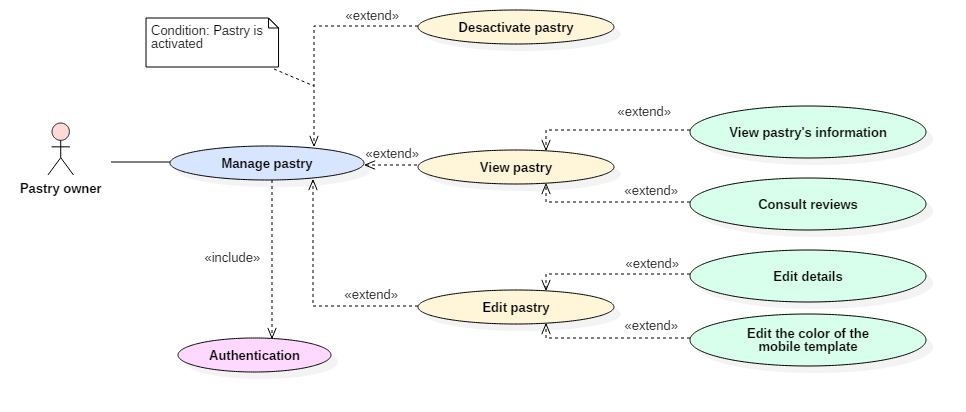
\includegraphics[width=7in,keepaspectratio]{usecasemanagepastry.png}
		\caption{Detailed use case: Manage his own clients}
		\label{user-case-manage-pastry}
	\end{figure}

\subsubsection*{Use case: Manage products}
Managing the list of products includes, viewing, editing and deleting the product as showing in Figure \ref{user-case-manage-products}
\begin{figure}[H]
	\centering
	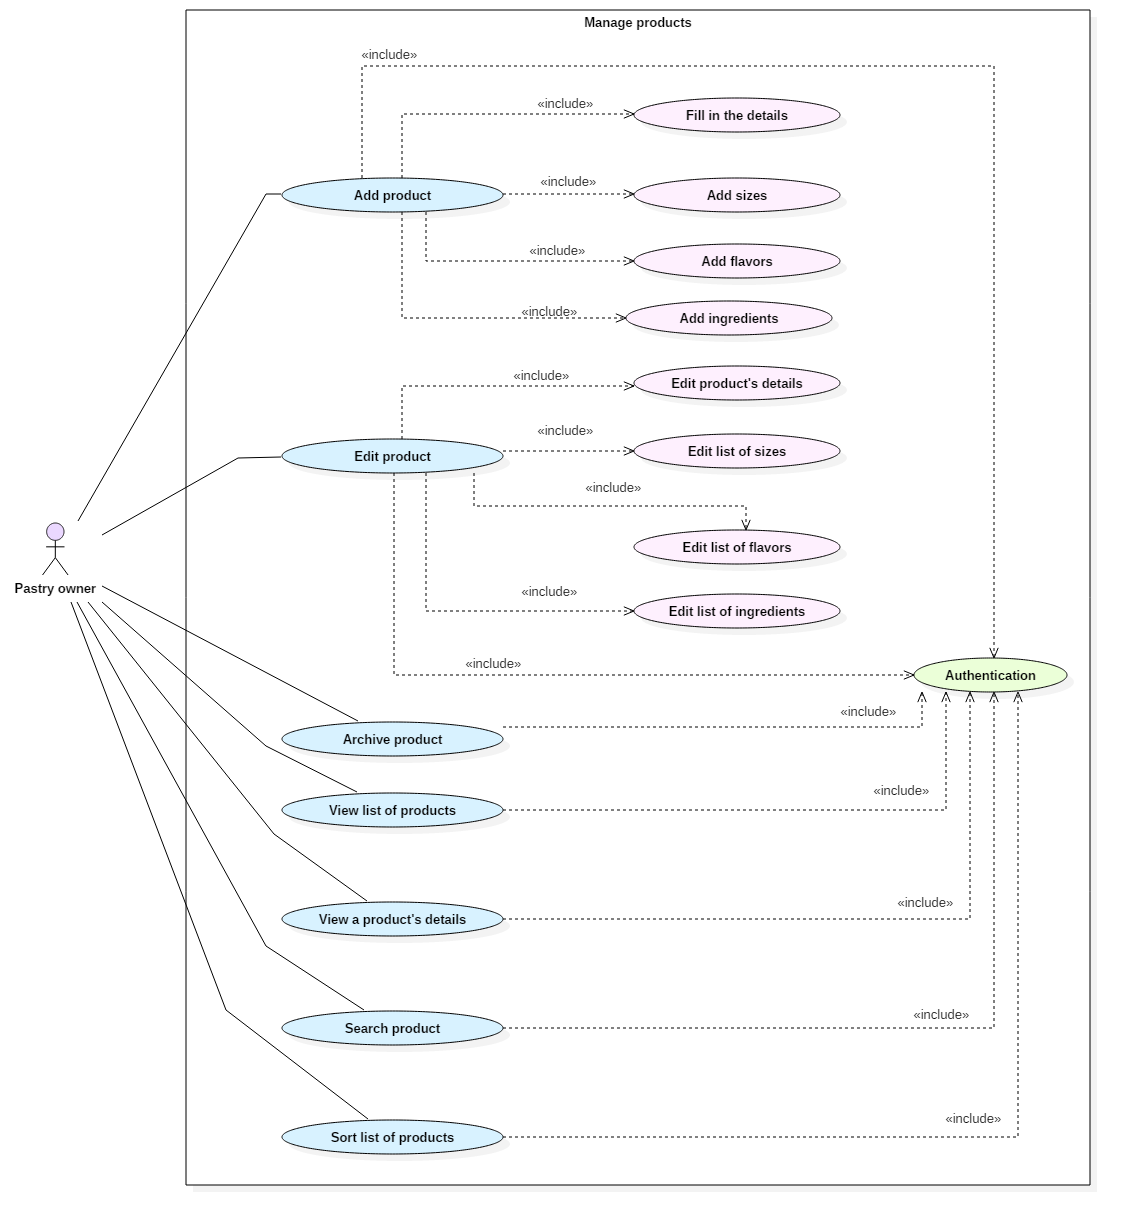
\includegraphics[width=6in,keepaspectratio]{manageproducts.png}
	\caption{Detailed use case: Manage products}
	\label{user-case-manage-products}
\end{figure}
	
	\subsection{Use case: Mobile}
		\subsubsection{General use case}
		\begin{figure}[H]
			\centering
			\includegraphics[width=7in,keepaspectratio]{UseCasemobile.png}
			\caption{General use case: Mobile}
			\label{user-case-mobile}
		\end{figure}
		\subsubsection{Detailed use case}
	
	\section*{Conclusion}
	\addcontentsline{toc}{section}{Conclusion}
	
	
	
	\chapter{Conception}
	\section*{Introduction}
	\addcontentsline{toc}{section}{Introduction}
	
	In this second chapter we will dedicate it to the conception part, in which we will include our class diagram with a detailed explanation. Then, we will be adding different sequence diagrams with more explanation.
	\section{Architecture}
	\subsection{Mobile}
	\subsection{Web}
	
	
	\section{Class diagram}
	Class diagrams are one of the most useful types of diagrams in UML as they clearly map out the structure of a particular system by modeling its classes, attributes, operations, and relationships between objects.
	
	\begin{table}[H]
		\begin{center}
			
			\caption{\label{Class_explanation} Class diagram explanation}
			\captionsetup[table]{skip=10pt}
			\setlength\doublerulesep{0.5pt}
			\begin{tabular}{| l | p{12cm} |}
				\hline \hline\hline
				\rowcolor{LightCyan}
				\textbf{ Entities} & \textbf{Definition} \\ \hline\hline\hline
				User               &                     
				\vtop{\hbox{\strut The user can be the place owner, place manager or the foodies}}
				
				\\ \hline
				Place manager      &                     
				\vtop{\hbox{\strut The person who manges the place.}}
				
				\\ \hline
				Place owner        &                     
				\vtop{\hbox{\strut The person who owns the place.}}
				\\
				\hline
				Foodie             &                     
				\vtop{\hbox{\strut The person who will be attending the place.}}
				\\ \hline
				Place              &                     
				\vtop{\hbox{\strut Places are added by the owner.}}
				\\ \hline
				Reservation        &                     
				\vtop{\hbox{\strut The foodie can book a dish in a place.}}
				\\ \hline
				Menu               &                     
				\vtop{\hbox{\strut The menu is composed from dishes.}}
				\\ \hline
				Dish               &                     
				\vtop{\hbox{\strut The food that a foodie will come for.}}
				\\ \hline
				Ingredient         &                     
				\vtop{\hbox{\strut A dish has ingredients.}}
				\\ \hline
				Likes/Dislikes     &                     
				\vtop{\hbox{\strut The foodie can like or dislike a place.}}
				\\ \hline
				Comments           &                     
				\vtop{\hbox{\strut The foodie can comment on a place.}}
				\\ \hline
				Rating             &                     
				\vtop{\hbox{\strut The foodie can give the place a rating.}}
				\\ \hline
				Offer              &                     
				\vtop{\hbox{\strut A place can make an offer.}}
				\\ \hline
				Location           &                     
				\vtop{\hbox{\strut A place has a location.}}
				\\ \hline
				
				
				
			\end{tabular}
			
		\end{center}
		
	\end{table}
	\clearpage
	\begin{figure}[H]
		\centering
		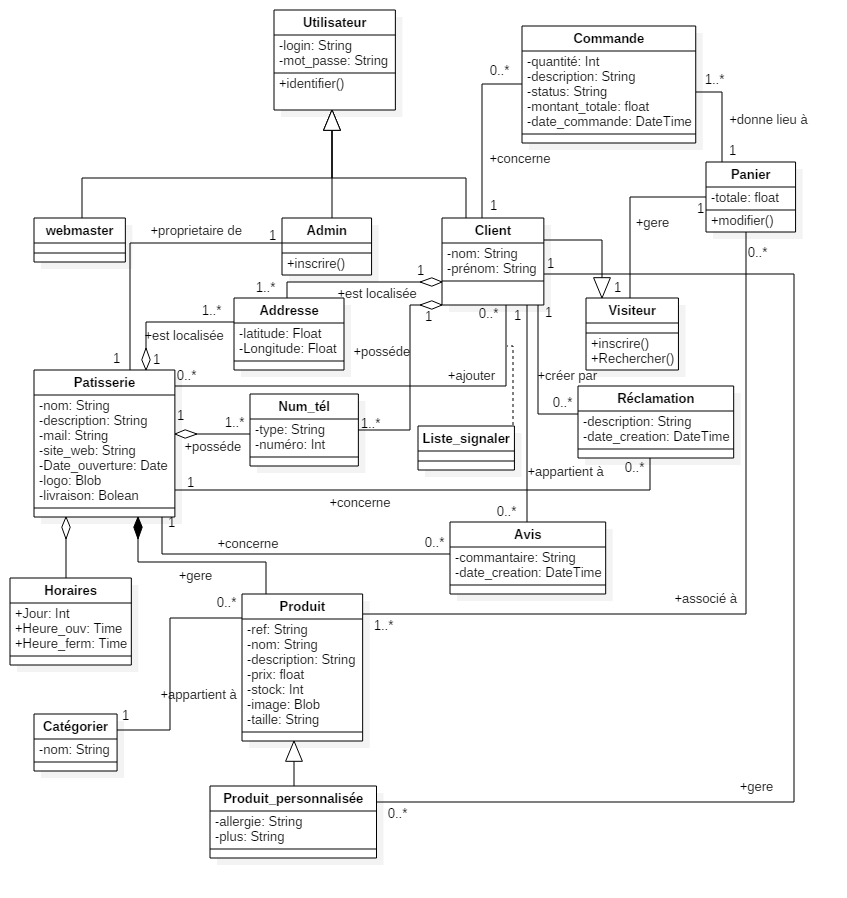
\includegraphics[width=6.8in,keepaspectratio]{class.png}
		\caption{Class Diagram}
	\end{figure}
	
	\clearpage
	\section{Interaction sequence diagram}
	A sequence diagram (SD) is a type of interaction diagram because it describes how and in what order a group of objects works together. These diagrams are used by software developers and business professionals to understand requirements for a new system or to document an existing process. Sequence diagrams are sometimes known as event diagrams or event scenarios.
	\subsection{Web}
	\subsection{Mobile}
	
	\section*{Conclusion}
	\addcontentsline{toc}{section}{Conclusion}
	Resuming this chapter, we ended up having a clearer vision about our objectives, now we pass on to the next chapter in which we will explain more about implementation.
	
	
	\chapter{Realization}
	\section*{Introduction}
	\addcontentsline{toc}{section}{Introduction}
	
	\section{Choice of the architecture}
	
	
	\section{Used technologies and frameworks}
	
	\section{Used software}
	
	
	\section{Implementation}
	\subsection{Web}
	\subsubsection{Shared interface}
	
	\subsubsection{Administrator's interface}
	
	\subsubsection{Bakery manager's interface}
	
	\subsection{Mobile}
	
	
	\section*{Conclusion}
	\addcontentsline{toc}{section}{Conclusion}
	To finalize this chapter, we ended having a clearer vision about the different functionalities, which will guide us to end up this project report with a conclusion summing up what we did, finalizing it with  our perspectives.	
	
	
	\chapter*{\centering General conclusion}
	\addcontentsline{toc}{chapter}{General conclusion}
	
	
	
	\clearpage
	\addcontentsline{toc}{chapter}{Bibliography}
	\bibliography{oxford}
	\bibliographystyle{ieeetr}
	

	
	\chapter*{\centering Appendix}
	\addcontentsline{toc}{chapter}{Appendix}
	
	

	
\end{document}